\FloatBarrier
\section*{Introduction}

I chose to address prompt 1, ``create and test an object/device that addresses a need or problem in your field of study,'' for my final project. I created a mock satellite with a solar panel and a sun sensor. The satellite rotates on two axes to point its solar panel in the direction of the sun as detected by the sun sensor. The completed build is shown in Figure~\ref{fig:satellite-completed}.
\begin{figure}[!ht]
    \centering
    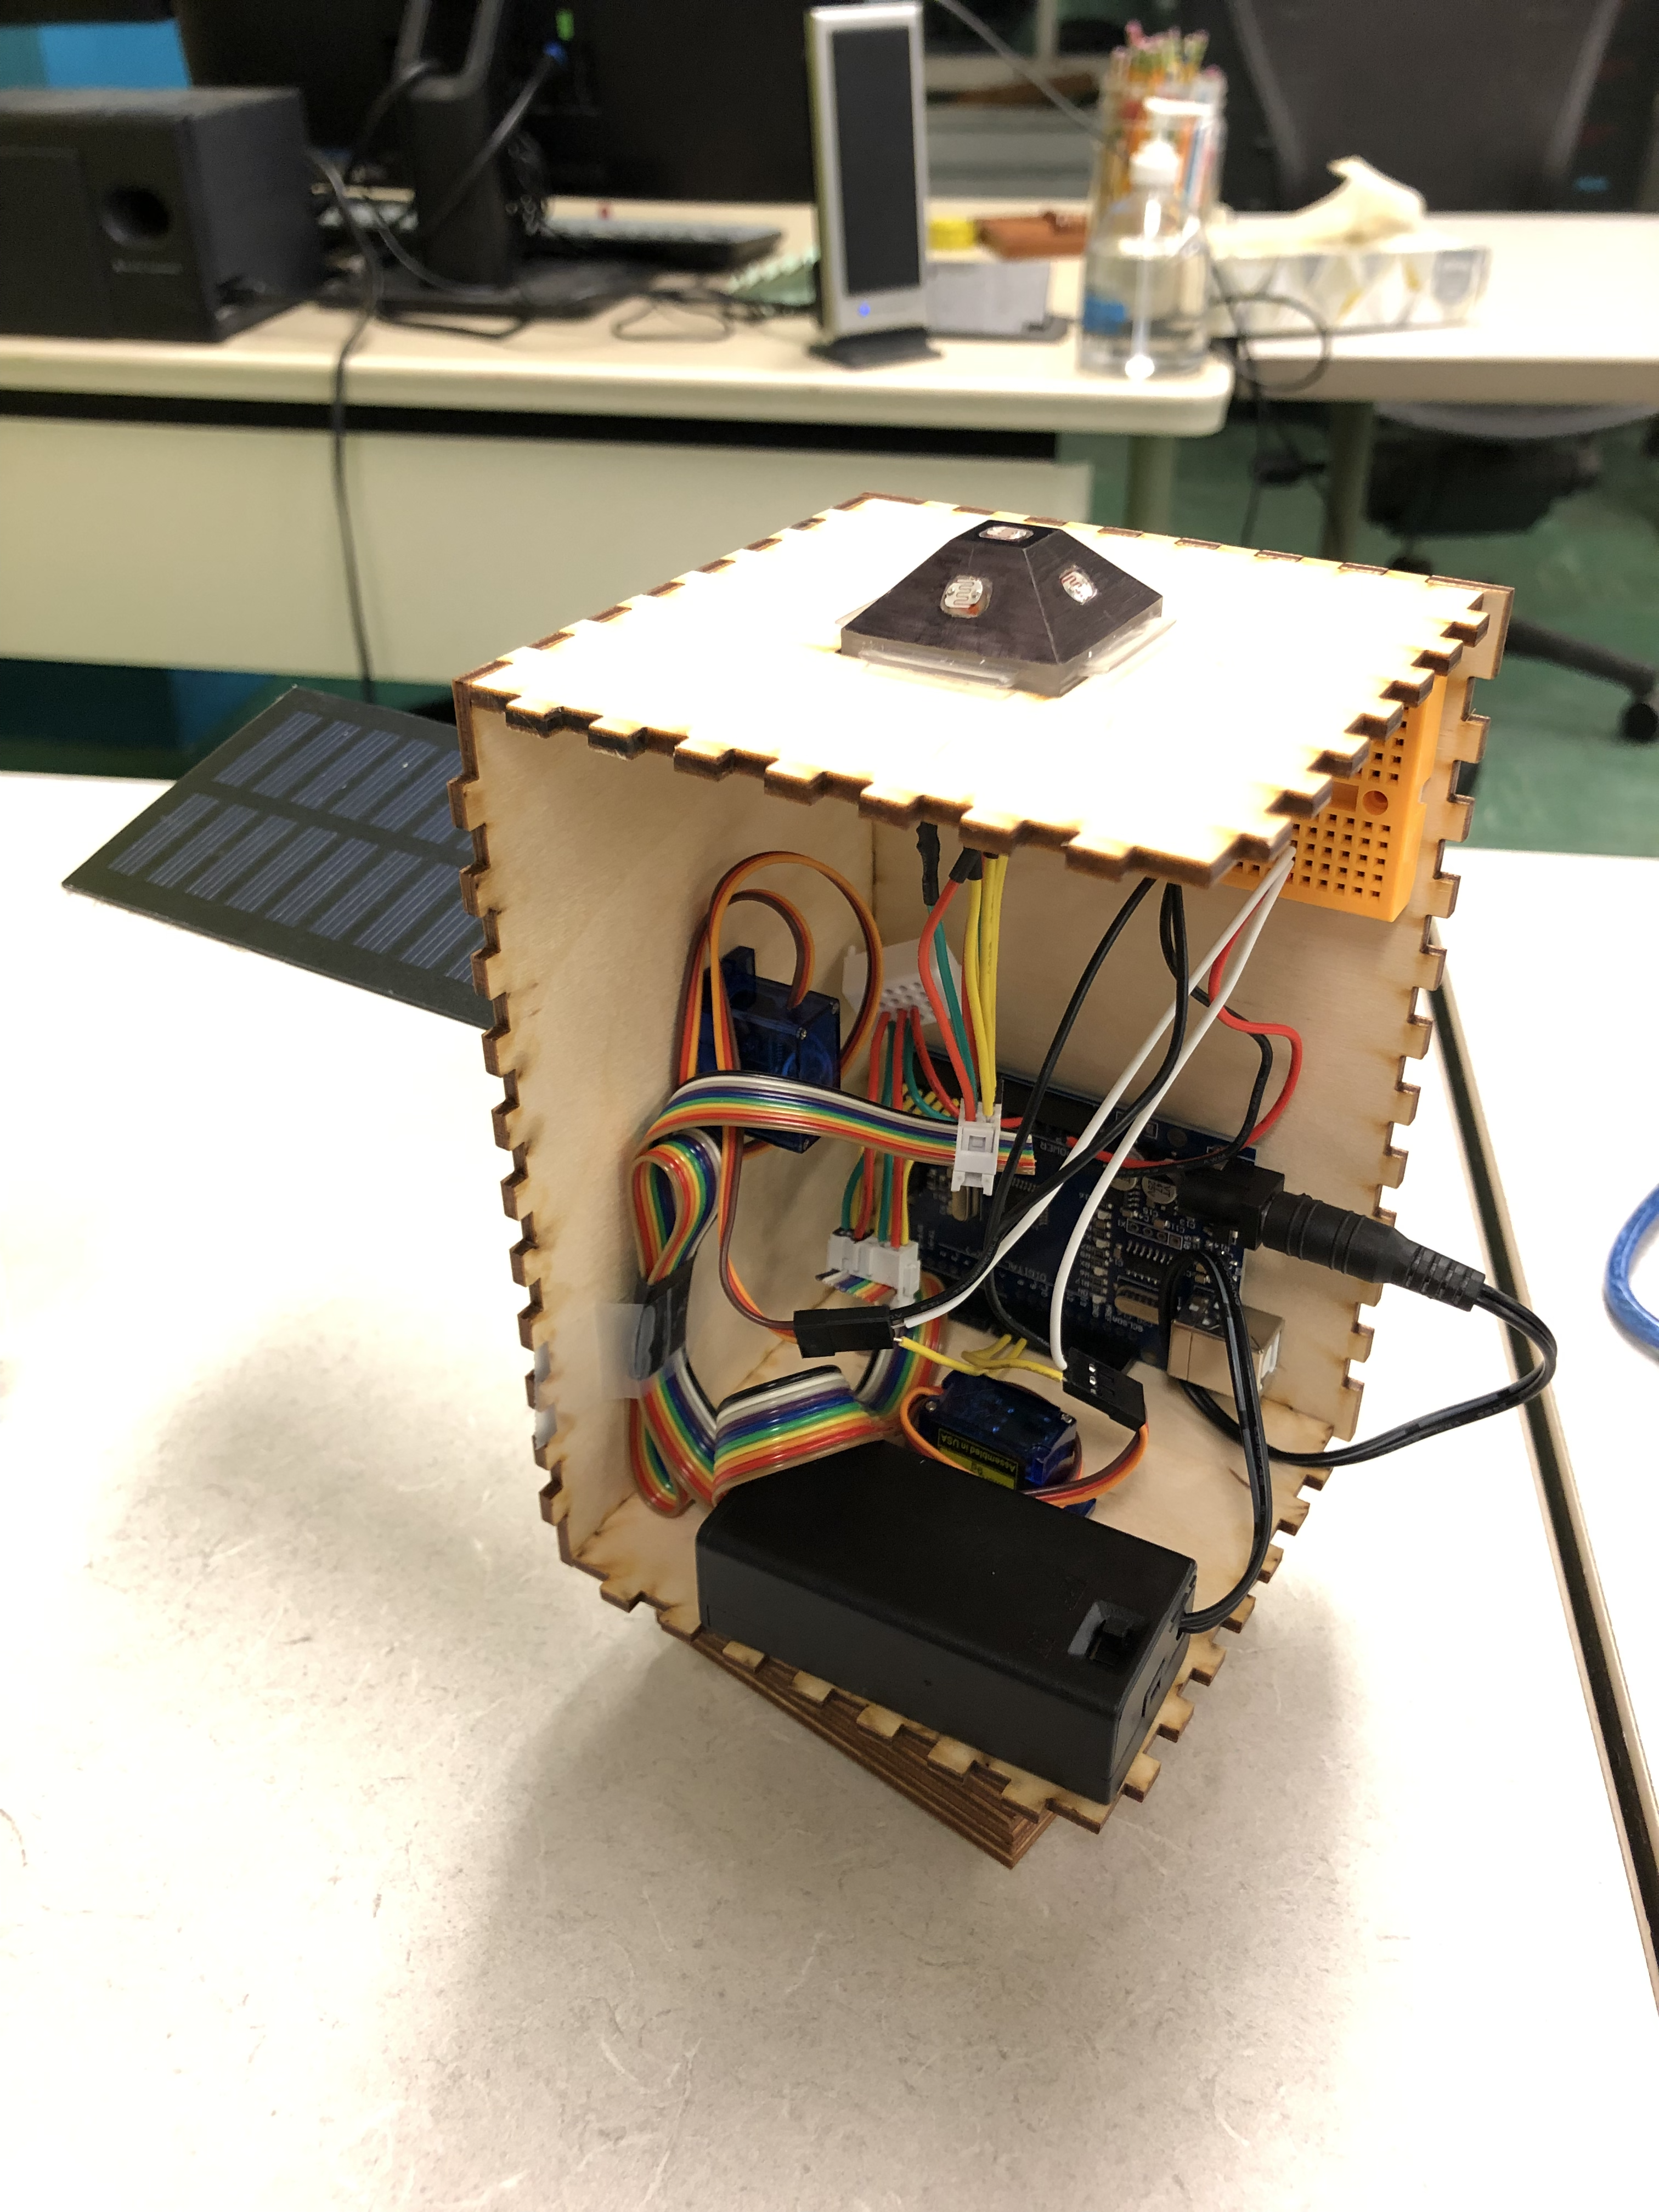
\includegraphics[width=0.55\linewidth]{figures/satellite-completed.png}
    \caption{Completed mock satellite with internals shown.}
    \label{fig:satellite-completed}
\end{figure}

Hundreds of satellites are launched every year into space to conduct scientific research, provide communications services, and more. Almost all satellites are solar-powered, and those satellites must be able to point their solar panels toward the Sun. Unlike on Earth, there is no atmosphere in space to refract the sunlight, so precise pointing is required for the solar panels to receive the maximum amount of energy and power the satellite. 



\section*{Sun Sensor Design}

The most challenging part of the project was the design and manufacturing of the sun sensor. A sun sensor measures the intensity of light in multiple directions and uses that information to calculate the direction of the sun. For my sun sensor design, I chose to use a truncated pyramid with sensors on each face excluding the bottom, which would give five different measurement directions. I planned to mount photoresistors on each face for light intensity detection. 

I created a sun sensor design in Fusion 360, shown in Figure~\ref{fig:sun-sensor-wireframe}. I wanted the sensor to be compact and robust --- since photoresistors are somewhat flimsy, I made slots on the faces for the photoresistors to fit into, along with channels for the leads.
\begin{figure}[!ht]
    \centering
    \includegraphics[width=0.8\linewidth]{figures/sun-sensor-wireframe.PNG}
    \caption{Wireframe view of the sun sensor design.}
    \label{fig:sun-sensor-wireframe}
\end{figure}

Since the design had many small details and hollow internals, I used resin printing instead of 3D printing. Surprisingly, the design worked on my first try. The resulting print with photoresistors is shown in Figure~\ref{fig:sun-sensor-pre-solder}. 

My design could have been improved in at least two ways. The four flanges coming out of each side of the sensor were printed without support, so the first few layers peeled off. The flanges are used to support the weight of the sun sensor when mounted in the satellite, so would have been better to make them more robust. 

Additionally, the channels inside the sun sensor were rather small, so there was a risk of the photoresistor leads touching each other, which would have shorted the sensor. I addressed this issue by adding small pieces of plywood between the leads to keep them separated. A better solution would have been to create separate channels for each of the positive and negative leads and reprint the sun sensor. 
\begin{figure}[!ht]
    \centering
    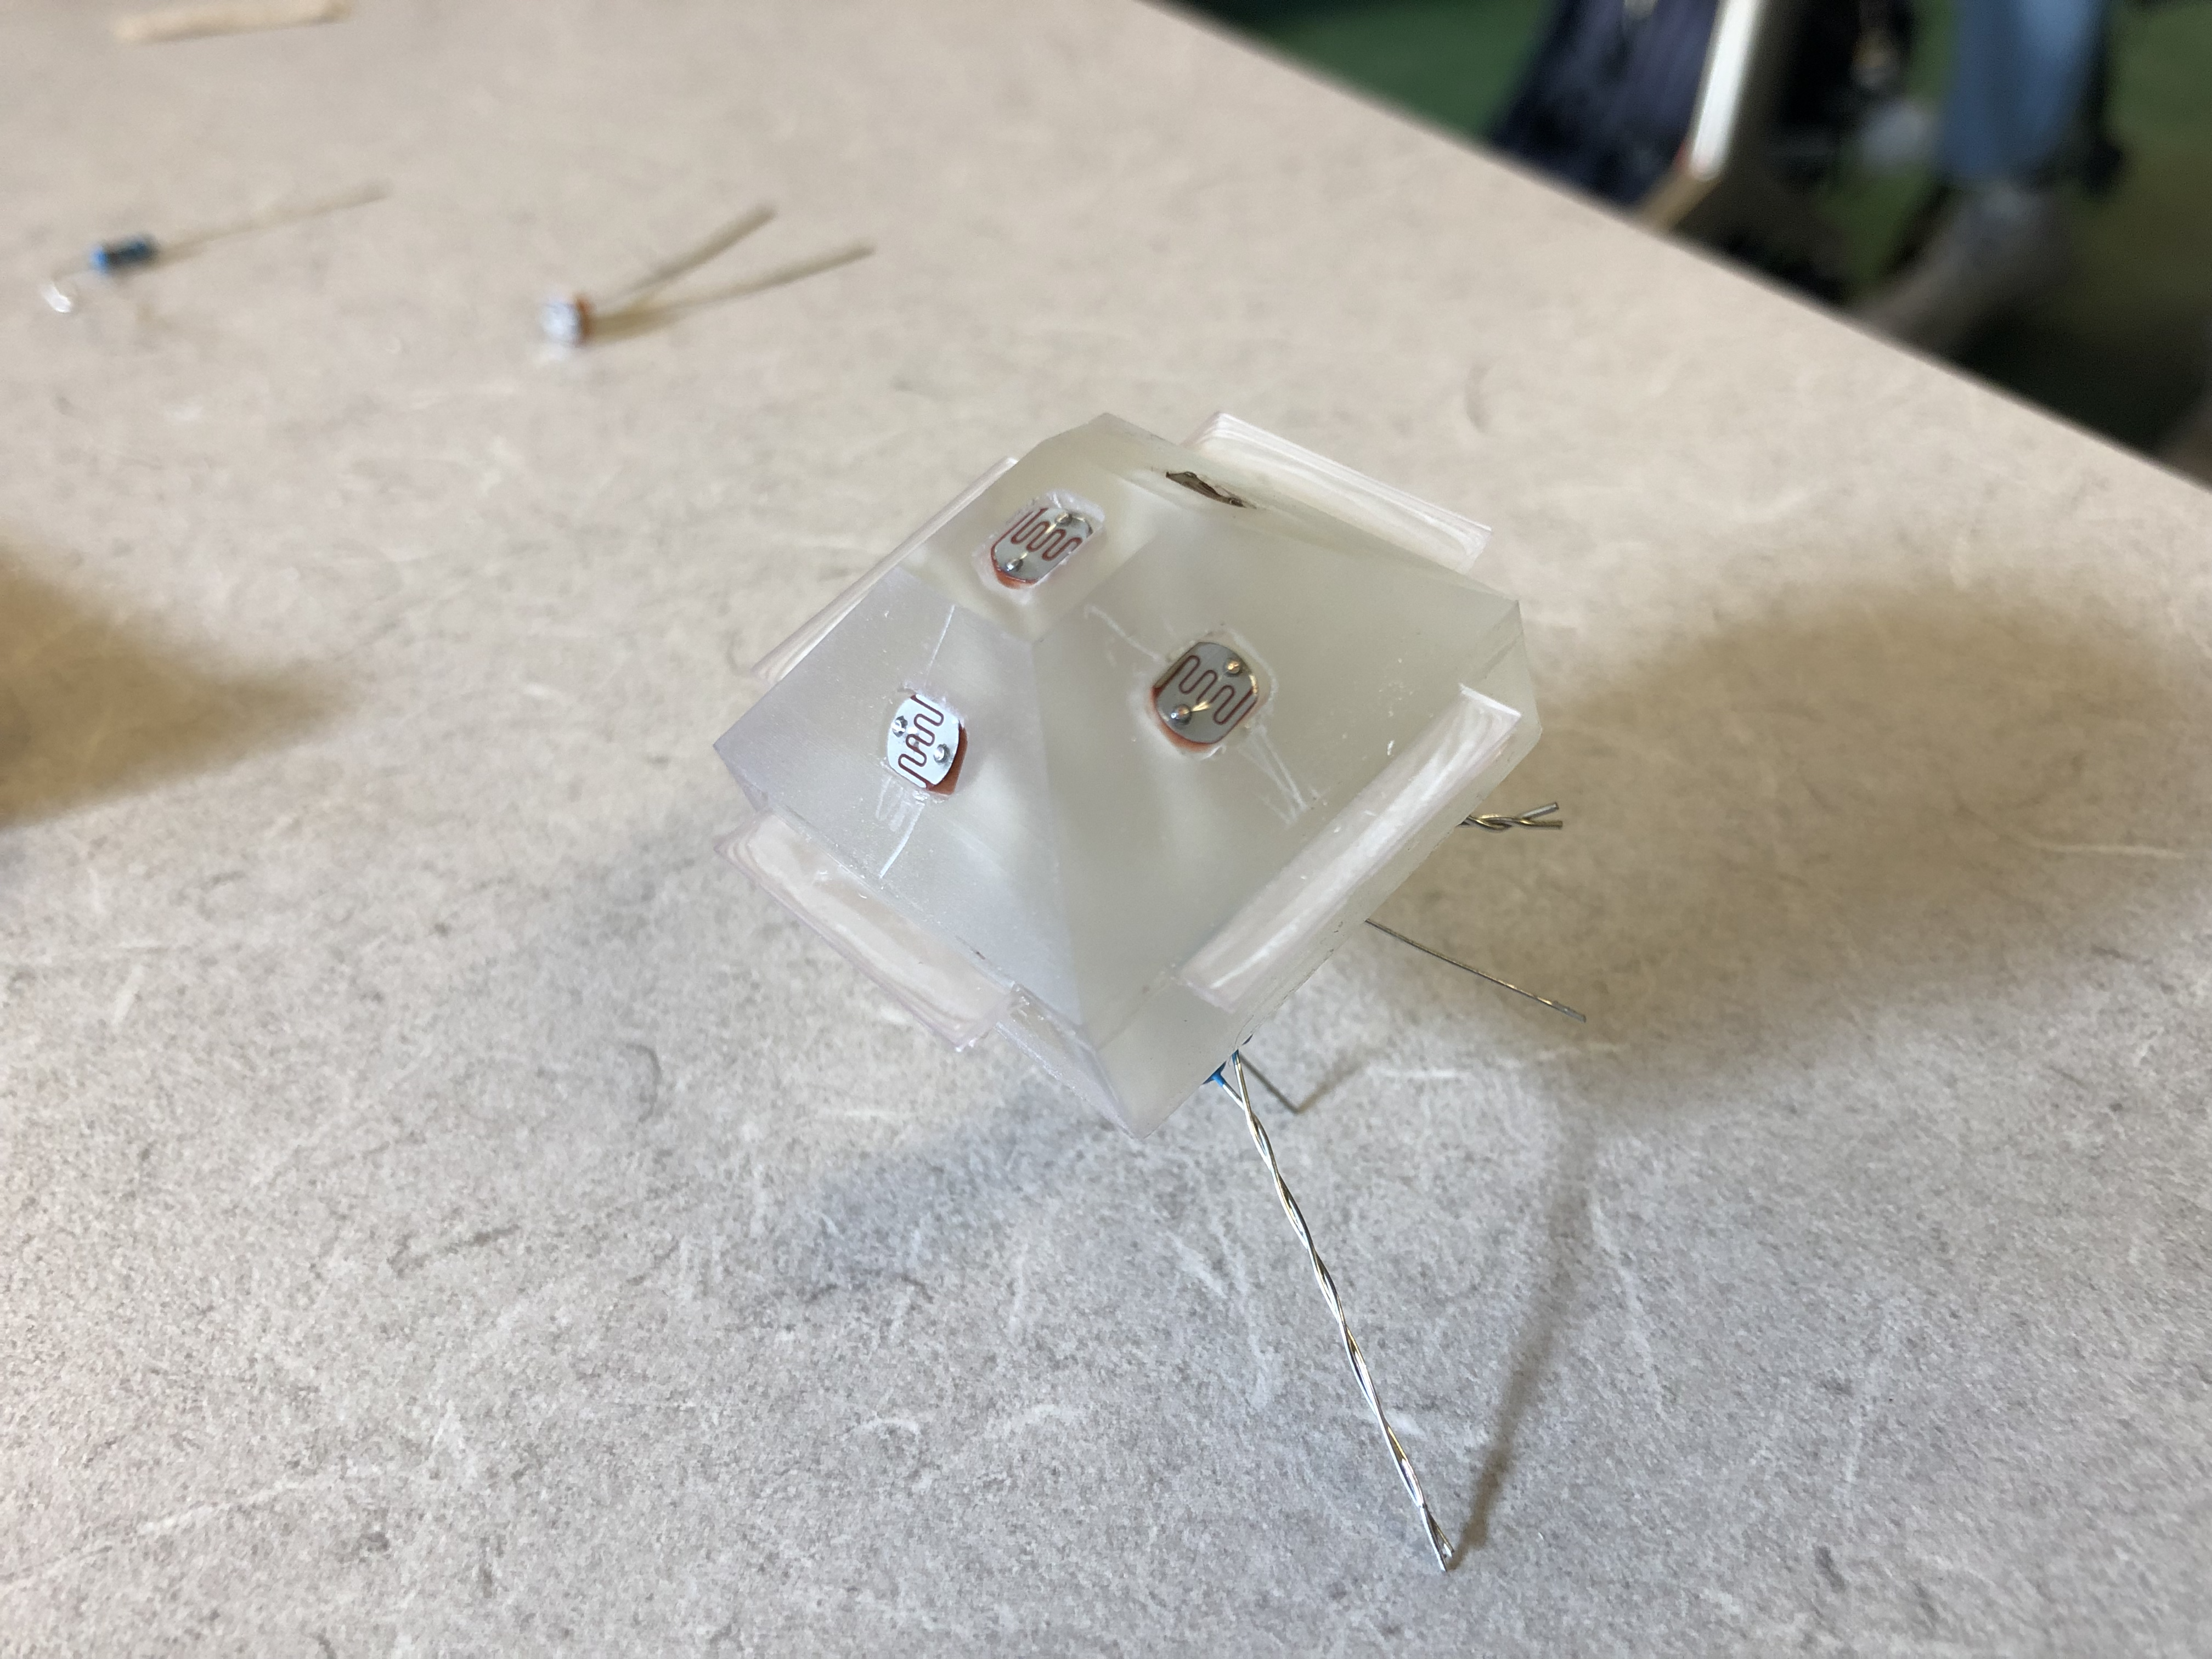
\includegraphics[width=0.8\linewidth]{figures/sun-sensor-pre-solder.png}
    \caption{Sun sensor resin print with photoresistors mounted.}
    \label{fig:sun-sensor-pre-solder}
\end{figure}

Next, I soldered resistors to each photoresistor, added heat-shrink tubing for insulation, and added a ribbon cable for easier interfacing with the Arduino. The result is shown in Figure~\ref{fig:sun-sensor-ribbon}. In hindsight, it would have been better to create a simple printed circuit board (PCB) to interface with the bottom of the sun sensor. This would have reduced the amount of soldering required and completely eliminated the need to braid wires together, making the design even more compact. 
\begin{figure}[!ht]
    \centering
    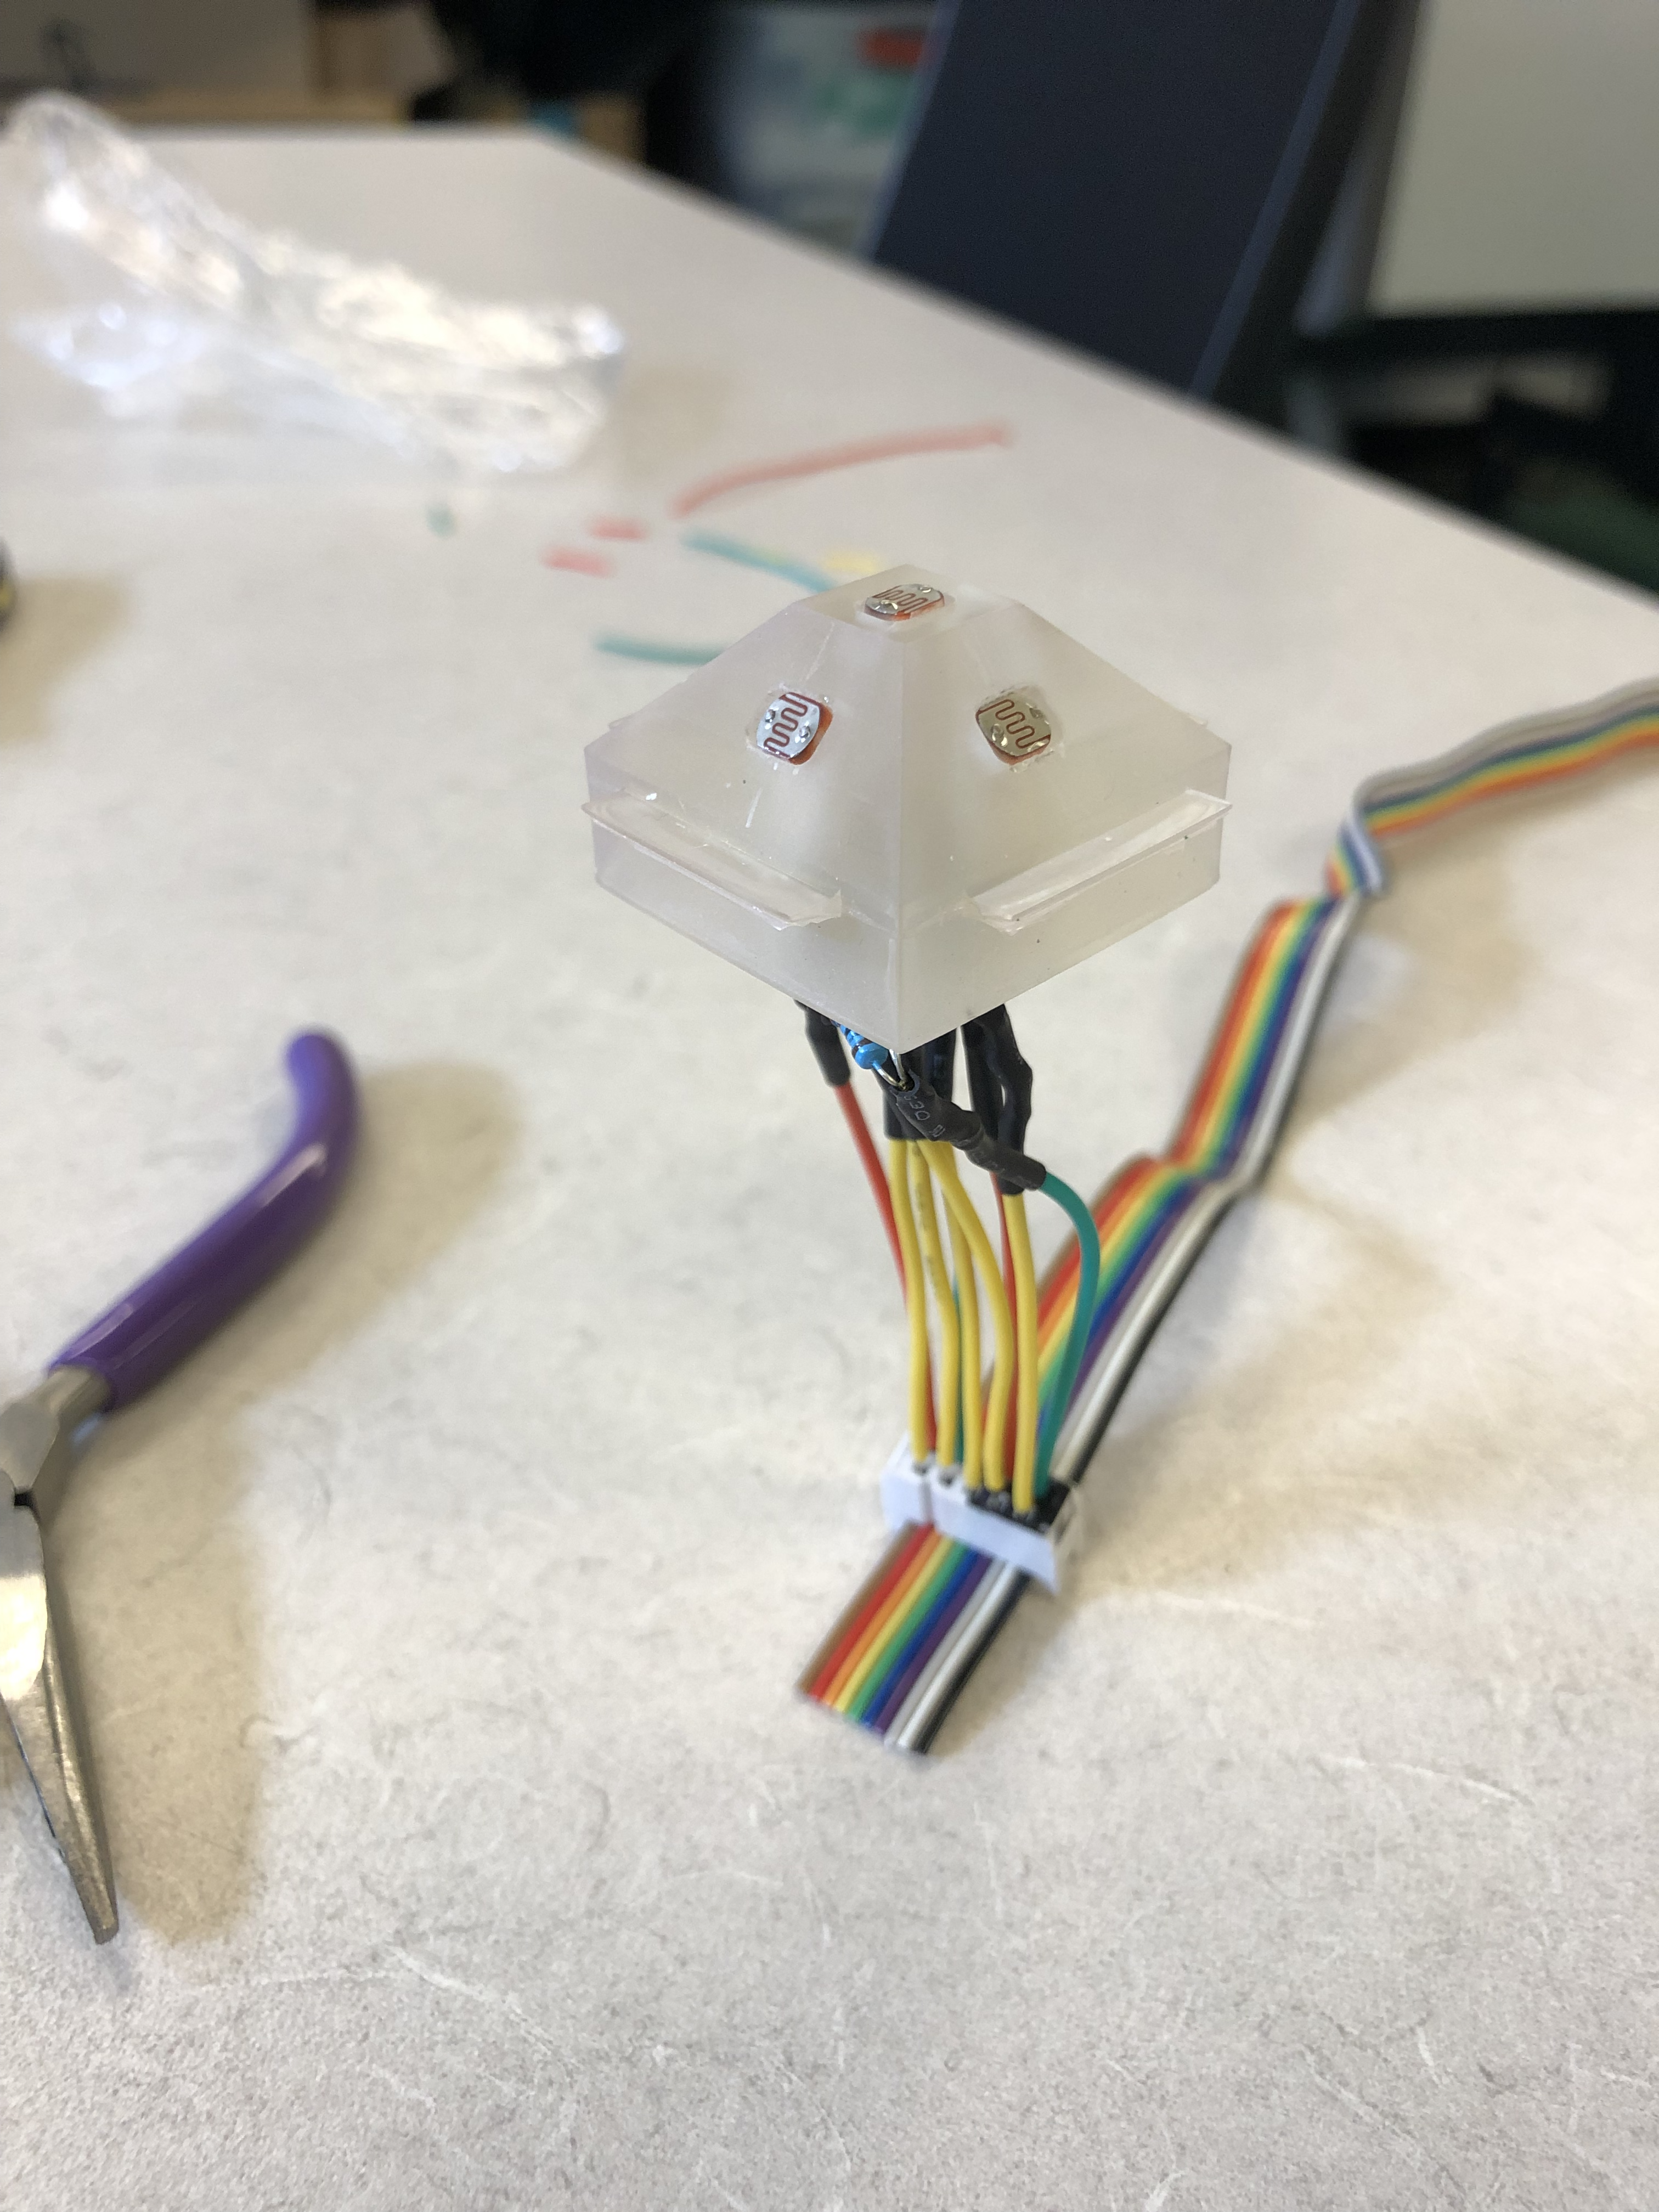
\includegraphics[width=0.55\linewidth]{figures/sun-sensor-ribbon.png}
    \caption{Completed sun sensor with ribbon cable attached.}
    \label{fig:sun-sensor-ribbon}
\end{figure}

Finally, I calibrated the sensors by measuring the output of each photoresistor while in near complete darkness and while under a bright flashlight, then wrote some Arduino code to test the functionality of the sun sensor. The finalized code is shown in Appendix A.



\section*{Build Hightlights}

The remainder of the build proceeded with very few issues, so only some hightlights are covered here. 

The mock satellite rotates on a stand using an SG90 servo. On my first attempt, I 3D printed an adapter for the servo arm, shown in Figure~\ref{fig:stand-3d-printed}. However, the servo had much more torque than I had anticipated but far less rigidity. Additionally, the stand had very little grip andd was far lighter than the rest of the satellite. The combination fo these factors meant that the servo would cause the base to rotate more than the satellite itself, and the satellite would lean heavily to one side. 
\begin{figure}[!ht]
    \centering
    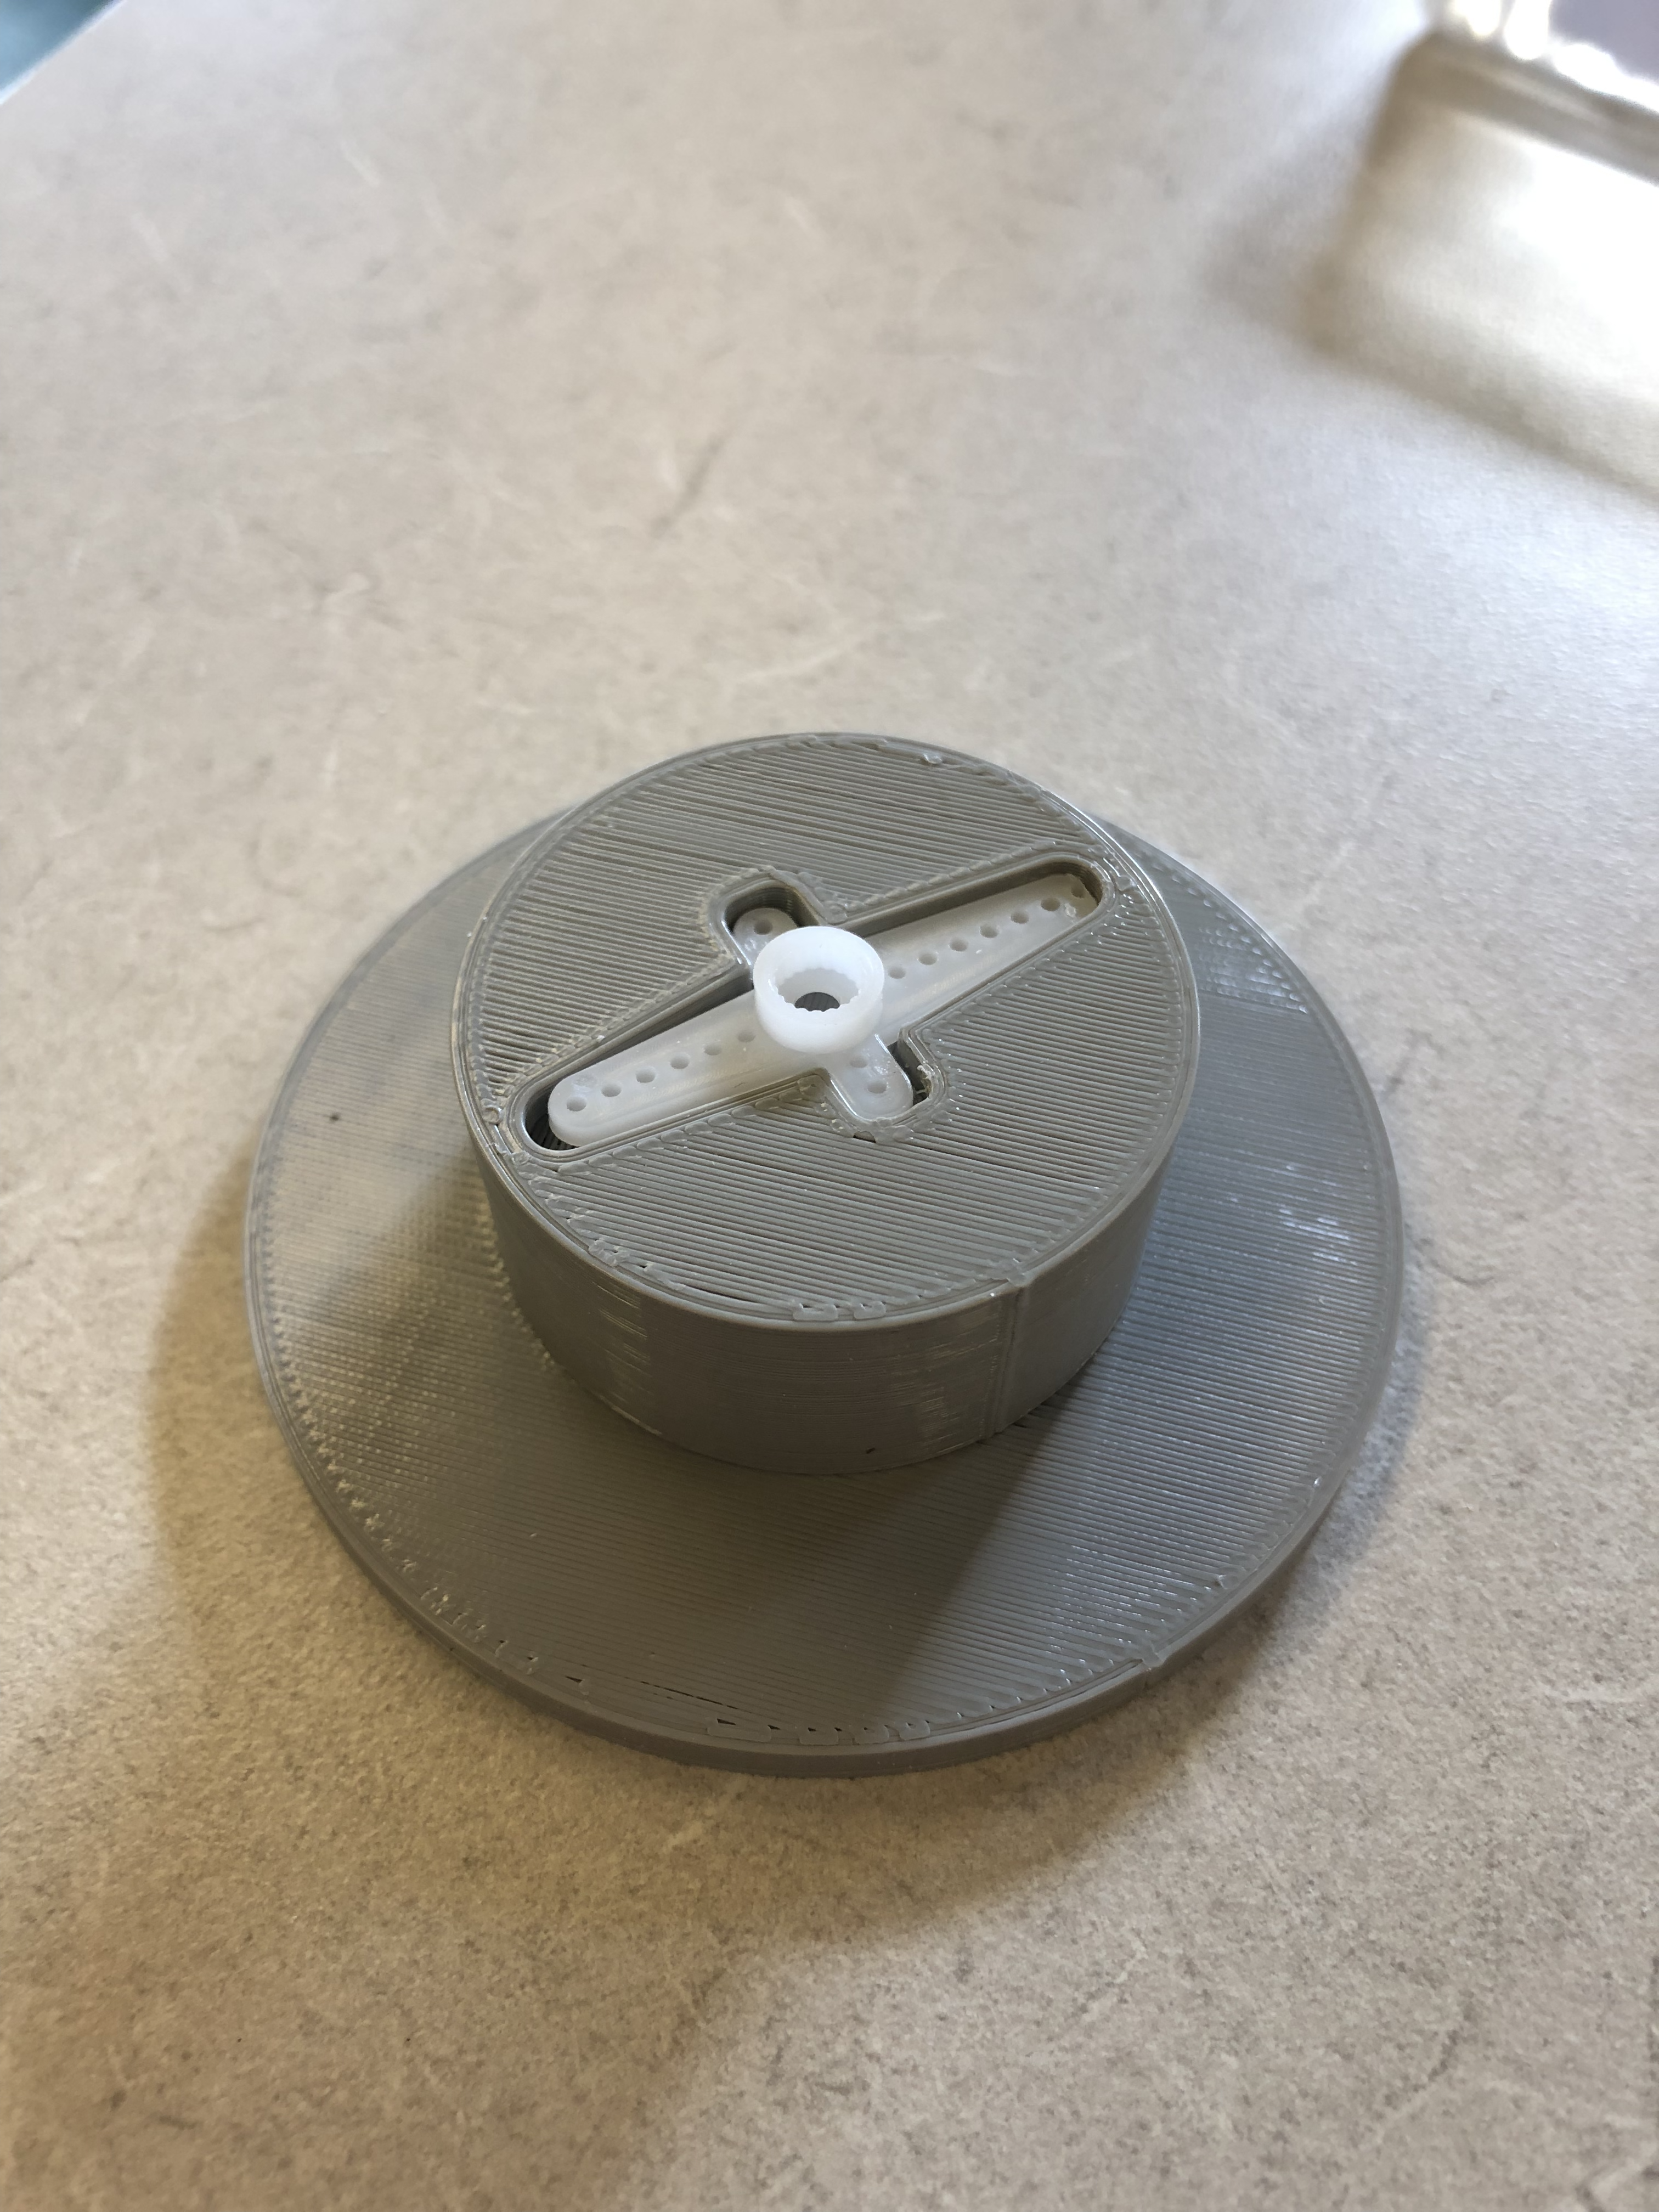
\includegraphics[width=0.55\linewidth]{figures/stand-3d-printed.png}
    \caption{First iteration of 3D-printed satellite stand. }
    \label{fig:stand-3d-printed}
\end{figure}

I improved the design by laser cutting several ploywood squares to fit over the existing stand. The plywood had holes to fit metal ball bearings so the satellite would by evenly supported. The improved stand is shown in Figure~\ref{fig:base-with-bearing-detached}.
\begin{figure}[!ht]
    \centering
    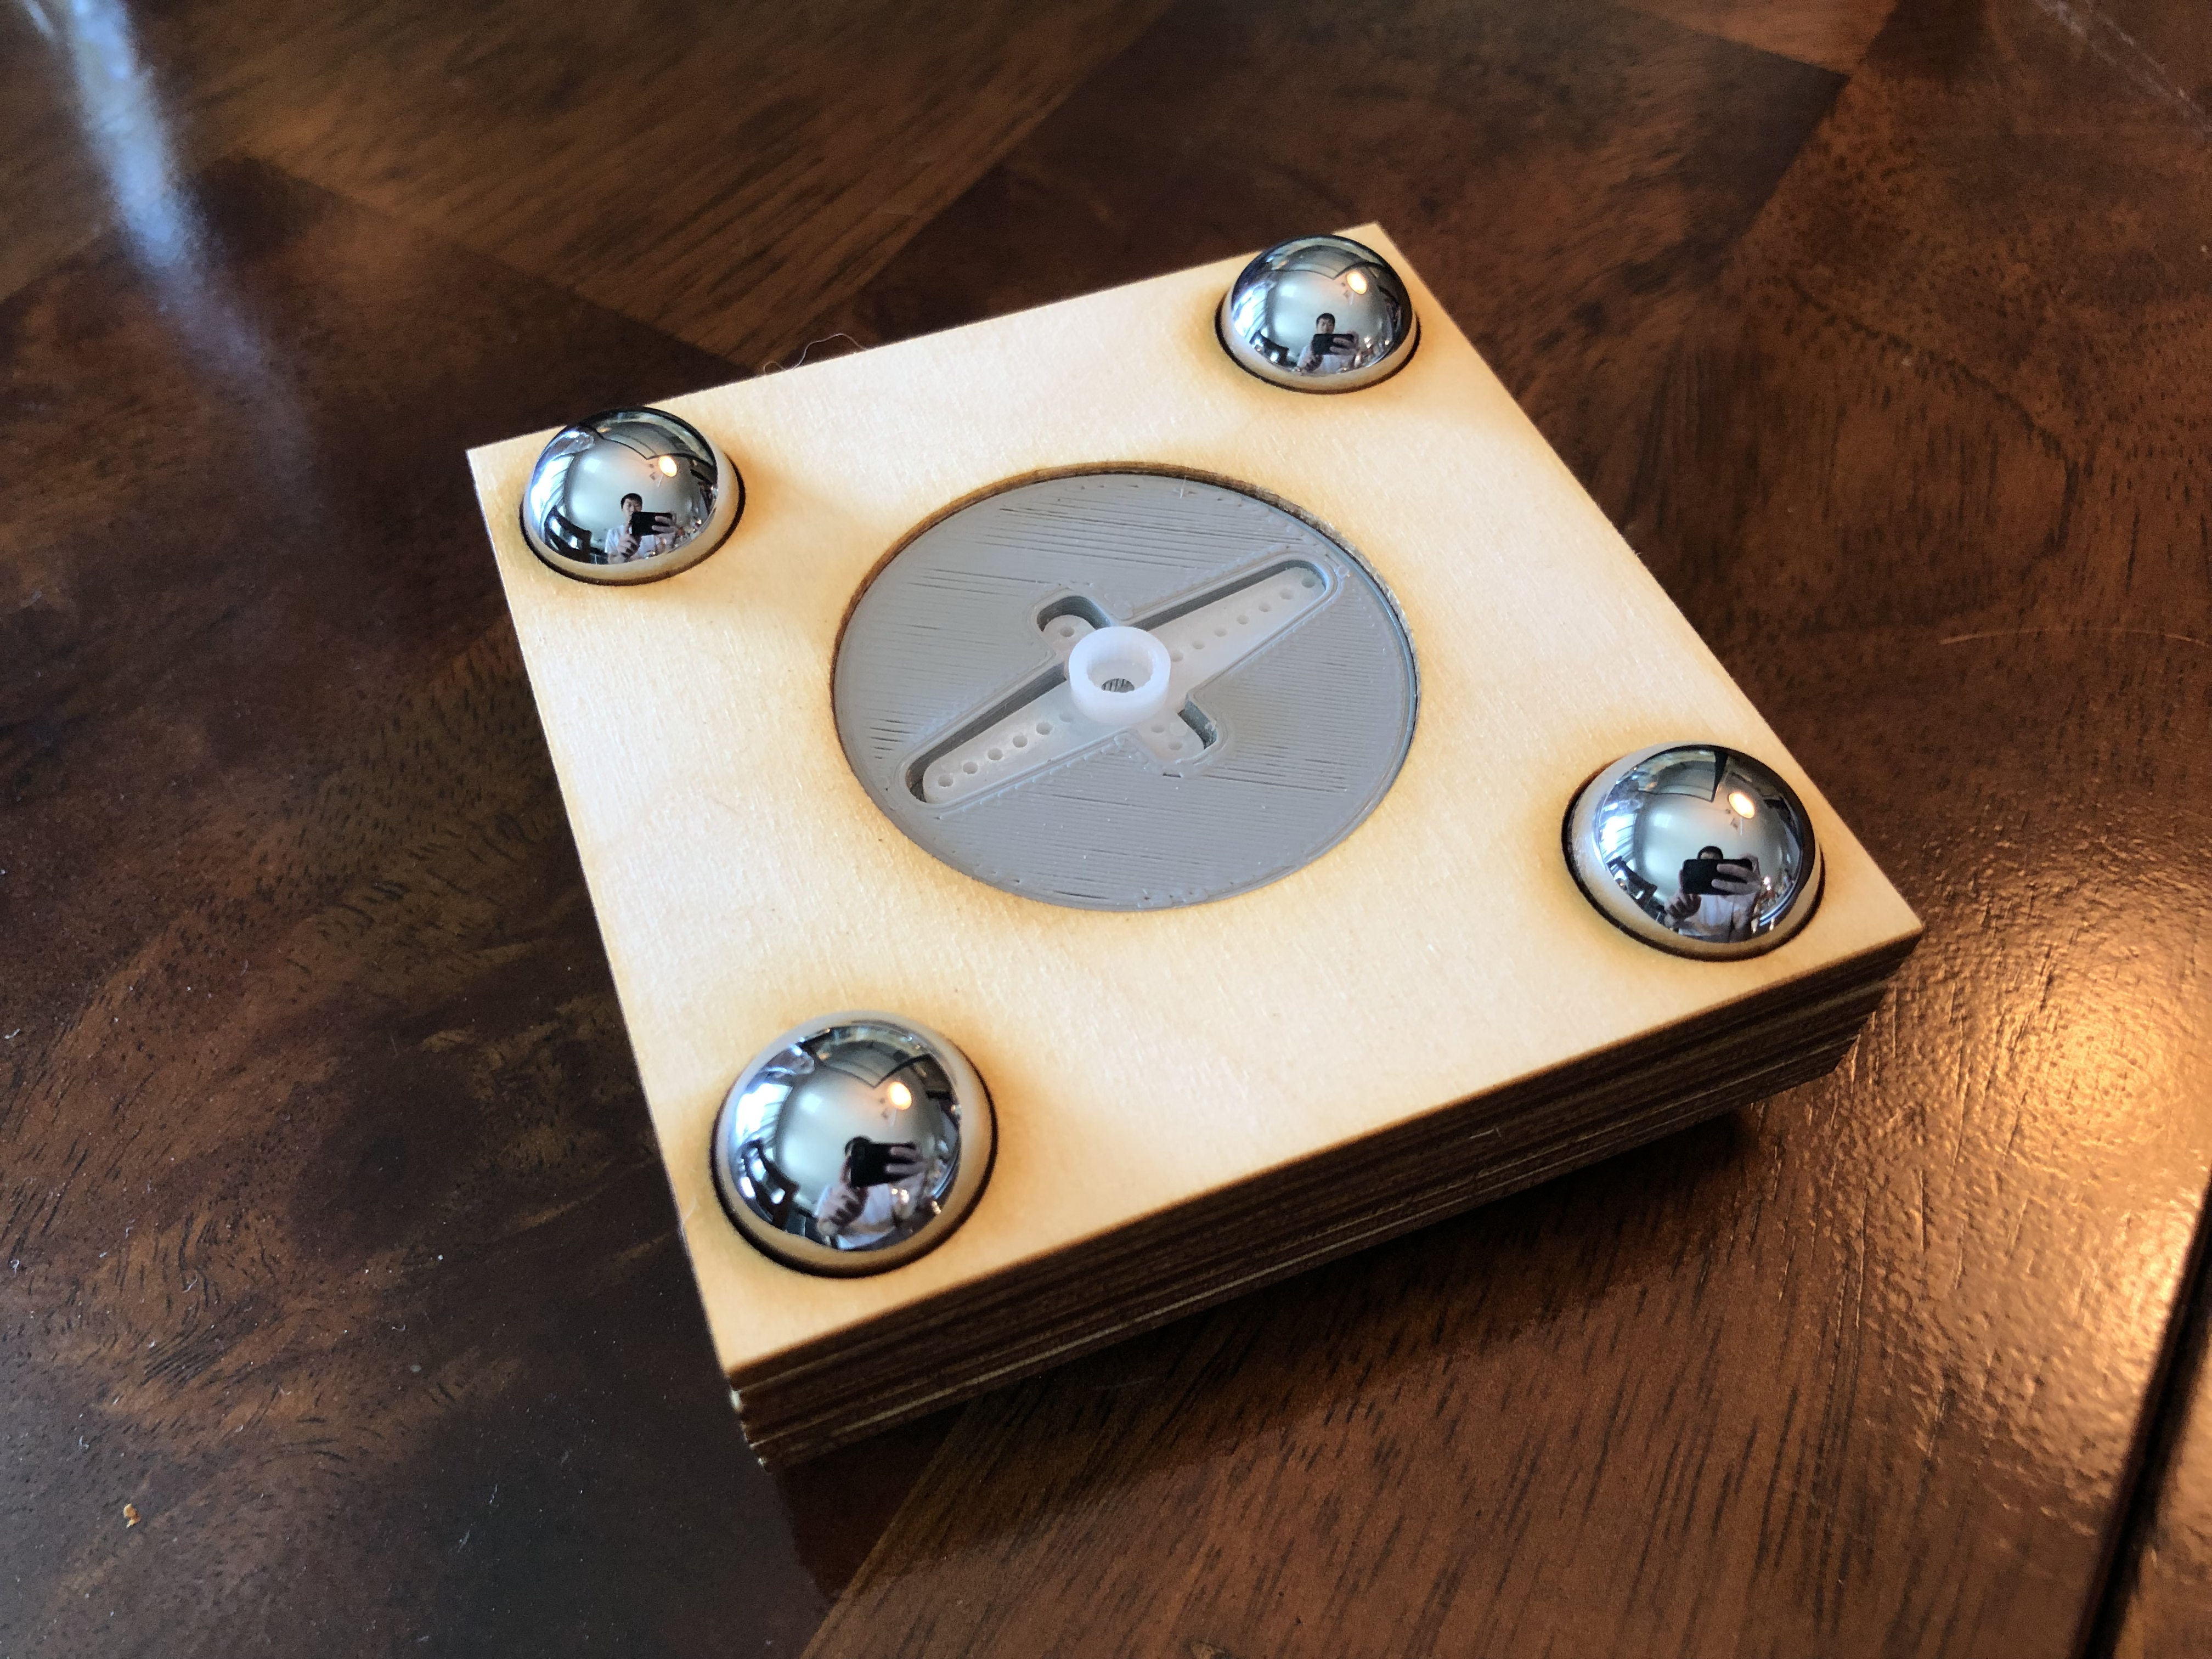
\includegraphics[width=0.8\linewidth]{figures/base-with-bearing-detached.png}
    \caption{Second iteration of the satellite stand with plywood and ball bearing support.}
    \label{fig:base-with-bearing-detached}
\end{figure}



\newpage
\section*{Appendix A}

\begin{lstlisting}
// REQUIRES the BasicLinearAlgebra library by Tom Stewart
#include <BasicLinearAlgebra.h>
#include <Servo.h>
#include <math.h>

using namespace BLA;

bool allowRotation = false;

const int pinW = A0;
const int pinC = A1;
const int pinN = A2;
const int pinS = A3;
const int pinE = A4;

const int delay_ms = 50;

const int baseServoPin = 9;
Servo baseServo;
float baseServoPos = 0;
float baseServoDesired = 0;
float baseServoTarget = 0;
const int baseServo_moving_window_size = 20;
const float baseServo_gain = 0.08;

const int panelServoPin = 10;
Servo panelServo;
float panelServoPos = 90;
float panelServoDesired = 90;
float panelServoTarget = 90;
const int panelServo_moving_window_size = 20;
const float panelServo_gain = 0.08;

const float Nmax = 600;
const float Smax = 500;
const float Emax = 600;
const float Wmax = 600;
const float Cmax = 600;

Matrix<5,3> A = {0, 1/sqrt(2), 1/sqrt(2),  // N
                 0, -1/sqrt(2), 1/sqrt(2), // S
                 1/sqrt(2), 0, 1/sqrt(2),  // E
                 -1/sqrt(2), 0, 1/sqrt(2), // W
                 0, 0, 1};
Matrix<3,5> AT = ~A;
Matrix<3,3> AtAinv = AT*A;
bool is_nonsingular = Invert(AtAinv);
Matrix<3,5> normalMat = AtAinv*AT;

Matrix<5,1> meas;
Matrix<3,1> sunDir;

float ra = 0;
float dec = 0;

void setup() {
  Serial.begin(9600);
  baseServo.attach(baseServoPin);
  panelServo.attach(panelServoPin);
}

void loop() {
  // measurements
  float valN = analogRead(pinN);
  float valS = analogRead(pinS);
  float valE = analogRead(pinE);
  float valW = analogRead(pinW);
  float valC = analogRead(pinC);

  // disable/enable rotation based on top signal
  if (valN < 20) {
    allowRotation = !allowRotation;
    delay(1000);
  }

  // compute sun angle
  meas = {valN/Nmax, valS/Smax, valE/Emax, valW/Wmax, valC/Cmax};
  sunDir = normalMat * meas;
  float mag = sqrt(sunDir(0)*sunDir(0)+sunDir(1)*sunDir(1)+sunDir(2)*sunDir(2));
  sunDir /= mag;
  ra = atan2(sunDir(1),sunDir(0)) / PI * 180;
  dec = asin(sunDir(2)) / PI * 180;
  
  // set satelite and solar panel angles
  baseServoDesired = boundAngle(baseServoPos + ra);
  if (baseServoDesired < 0) {
    baseServoDesired += 180;
    panelServoDesired = 90 - (90-dec);
  } else {
    panelServoDesired = 90 + (90-dec);
  }
  baseServoDesired = boundServoPosition(baseServoDesired);
  panelServoDesired = boundServoPosition(panelServoDesired);

  // smoothing
  baseServoTarget = baseServoTarget * (1.0 - 1.0/baseServo_moving_window_size);
  baseServoTarget += baseServoDesired / baseServo_moving_window_size;
  panelServoTarget = panelServoTarget * (1.0 - 1.0/panelServo_moving_window_size);
  panelServoTarget += panelServoDesired / panelServo_moving_window_size;

  // set rotation
  baseServoPos += baseServo_gain * (baseServoTarget - baseServoPos);
  panelServoPos += panelServo_gain * (panelServoTarget - panelServoPos);
  baseServoPos = boundServoPosition(baseServoPos);
  panelServoPos = boundServoPosition(panelServoPos);

  // command rotation
  if (allowRotation) {
    baseServo.write(baseServoPos);
    panelServo.write(panelServoPos);
  }

  delay(delay_ms);
}

float boundServoPosition(float servoPos) {
  if (servoPos > 180) { return 180; } 
  if (servoPos < 0)   { return 0; }
  return servoPos;
}

float boundAngle(float ang) {
  return fmod(ang+180, 360) - 180;
}

\end{lstlisting}